\documentclass[10pt]{beamer}
\usepackage{bm,caption,fontspec,minted,multirow,tabularx,xeCJK}
% \usepackage{listings}
\usetheme{AnnArbor}
\setCJKmainfont{SimSun}
\usemintedstyle{emacs}
\setbeamercolor{normal text}{bg=black!10}
\begin{document}
\newcommand{\minitab}[2][l]{\begin{tabular}{#1}#2\end{tabular}}
\title{Design of Integrated Microrobotic Fish}
% \newfontfamily\monaco{Monaco}
\subtitle{Presentation 4 - Physical Model (Improving) \& COMSOL Simulation (2D)}
\author{Yihua Liu}
\institute{UM-SJTU Joint Institute}
\date{March 16, 2021}
\maketitle
\begin{frame}{Contents}
    \tableofcontents
\end{frame}
\section{COMSOL Simulation (2D)}
\begin{frame}{COMSOL Simulation (2D)}{From KLayout to AutoCAD}
    \begin{figure}
        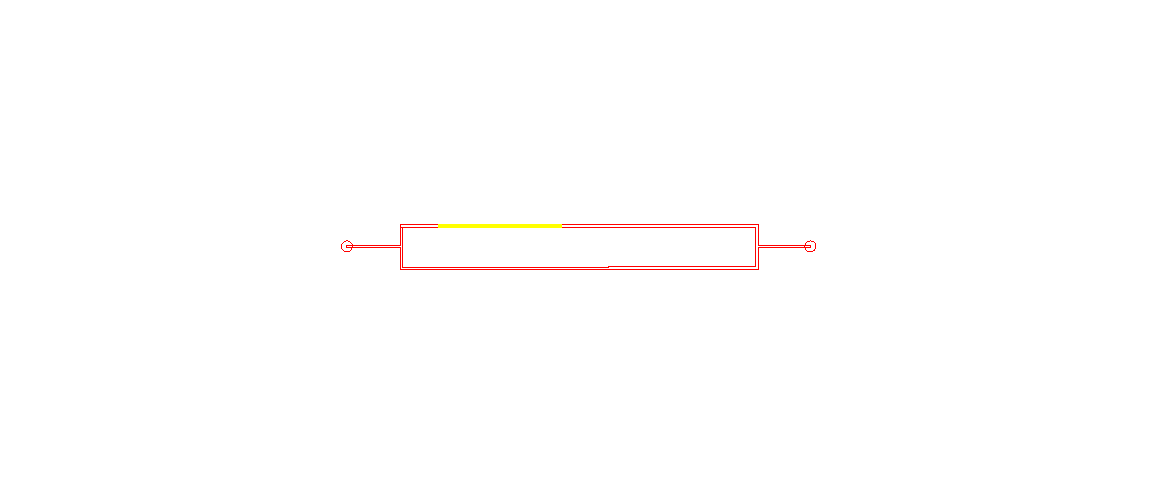
\includegraphics[width=\textwidth]{1.eps}
        \caption{The whole layout.}
    \end{figure}
\end{frame}
\begin{frame}{From KLayout to AutoCAD}{Details}
    \begin{figure}
        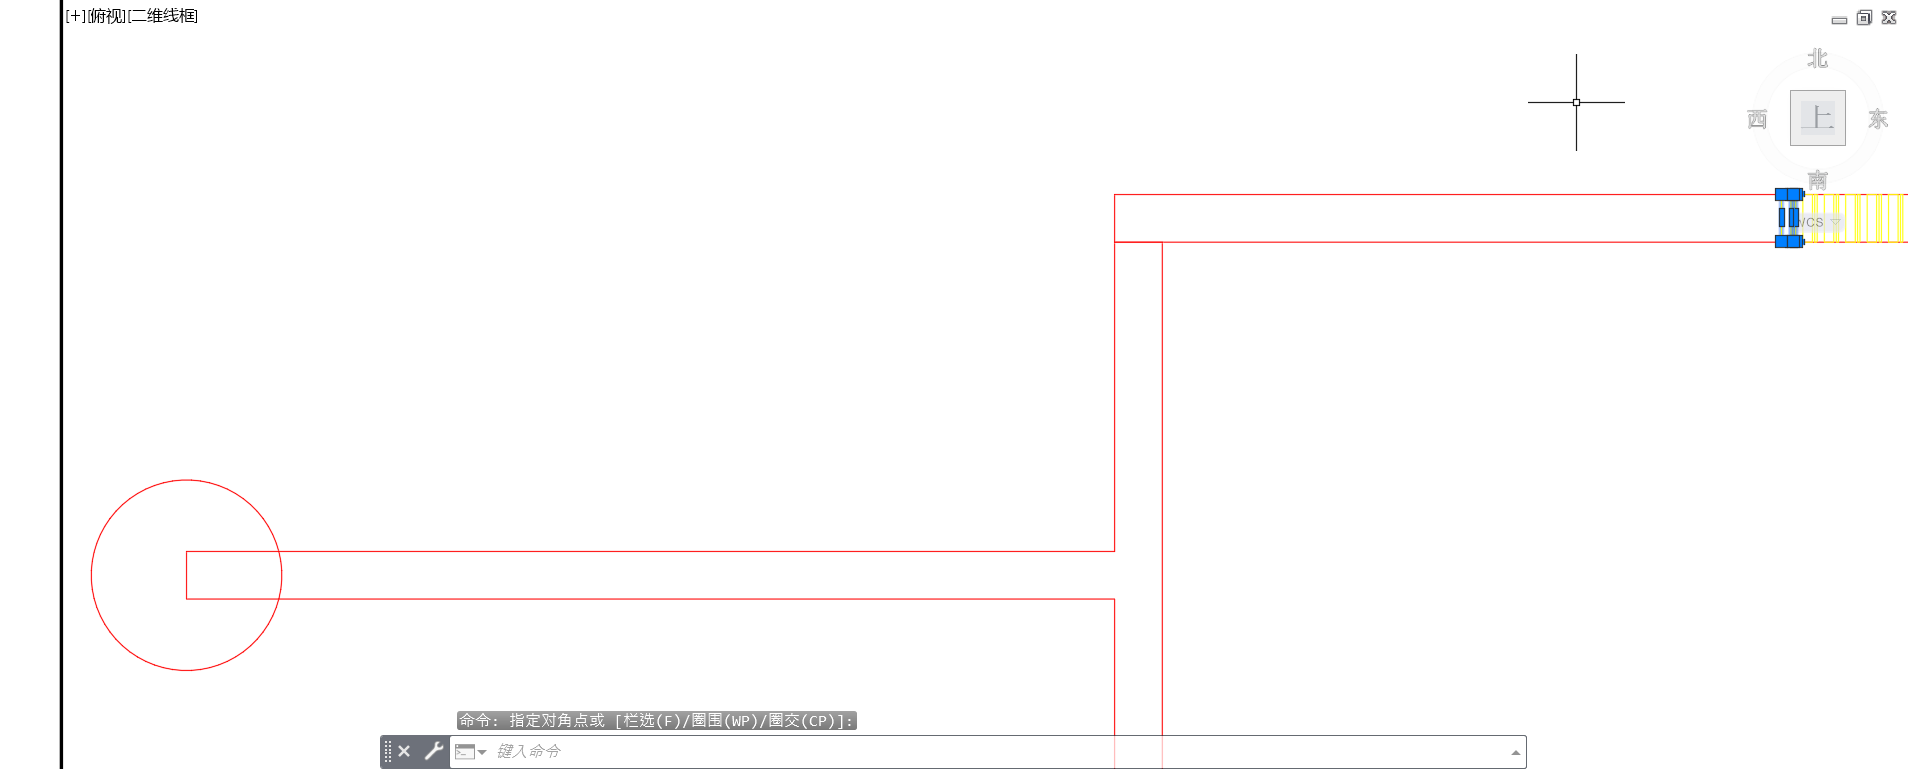
\includegraphics[width=\textwidth]{2.png}
        \caption{Details.}
    \end{figure}
\end{frame}
\begin{frame}{AutoCAD Processing}{Steps}
    \begin{enumerate}
        \item Erase the redundant boundaries.
        \item Erase the up, left, and right edges of the tiny rectangles.
        \item Erase the down edges of the tiny rectangles and redraw the startpoints and endpoints of the edges.
    \end{enumerate}
    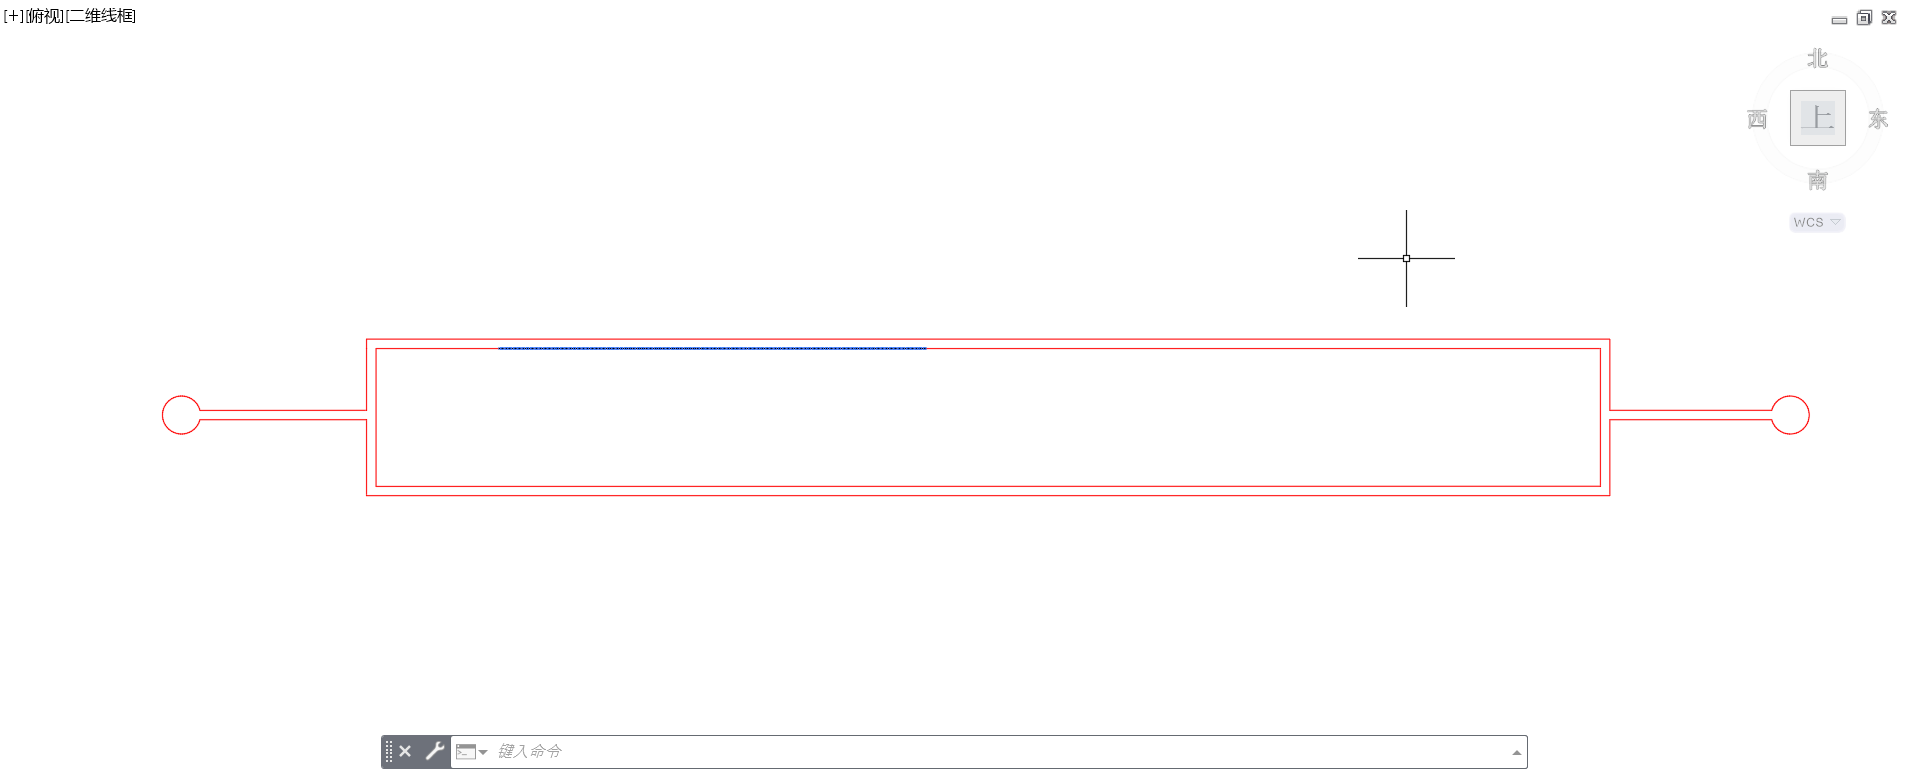
\includegraphics[width=\textwidth]{3.png}
\end{frame}
\begin{frame}[fragile]{AutoCAD Processing}{AutoLISP/Visual Lisp Code}
    % \lstinputlisting[basicstyle=\tiny,breaklines,frame=shadowbox,language=Lisp,numbers=left]{../Geometry/vertices_reserving.lsp}
    % \inputminted[breaklines,breakanywhere,fontsize=\tiny,frame=single]{../Geometry/vertices_reserving.lsp}
    \begin{minted}[breaklines,breakanywhere,fontsize=\tiny,frame=single]{newlisp}
; Inspired by https://forums.autodesk.com/t5/visual-lisp-autolisp-and-general/get-x-y-z-coordinates-of-vertices-of-multiple-3dpolylines/m-p/2822802/highlight/true#M292893
(defun c:test (/ ss cnt fn obj lst1 str)  ; Check parameters first, otherwise "错误: 参数类型错误: lselsetp nil" or "错误: 参数太多"
  (setq ss (ssget ":E" '((0 . "LINE")))  ; Exported electrodes are lines, not polylines; ":E" indicates selection set needed before running
    cnt -1
    fn (open "D:\\Documents\\Programming\\AutoLISP\\coordlist.txt" "w")  ; File operations are not necessary, just for checking
  )
  (repeat (sslength ss)
    (setq obj (vlax-ename->vla-object (ssname ss (setq cnt (1+ cnt)))))
    (if
      (= "AcDbLine" (vlax-get obj 'Objectname))  ; Alternatively ((eq (vla-get-ObjectName obj) "AcDbLine")
      (progn
        (setq sp (vlax-get obj 'StartPoint)  ; Alternatively (setq sp (vlax-curve-getstartpoint obj))
          ep (vlax-get obj 'EndPoint)  ; Alternatively (setq ep (vlax-curve-getendpoint obj))
          ; Note that different from "AcDbPolyline", "AcDbLine" does not have "Coordinates", otherwise "错误: ActiveX 服务器返回错误: 未知名称: "COORDINATES""
          str (strcat (rtos (car sp)) "," (rtos (cadr sp)) ";" (rtos (car ep)) "," (rtos (cadr ep)) ";")
          ; Here must be "cadr" rather than "cdr", otherwise "错误: 参数类型错误: numberp: (1300.0 0.0)"
          ; Remember don't concatenate str without initializing it by (setq str ""), otherwise "错误: 参数类型错误: stringp nil"
          mspace (vla-get-modelspace 
            (vla-get-activedocument 
              (vlax-get-acad-object)
            )
          )
        )
        (write-line str fn)
        (vla-addpoint mspace (vlax-3d-point sp))  ; (command "Point" sp ep)
        (vla-addpoint mspace (vlax-3d-point ep))  ; (vla-put -INSERTIONPOINT Obj mypoint) (vlax-put Obj 'INSERTIONPOINT mypoint)
        (vla-delete obj)  ; (command "Erase" obj)
      )
    \end{minted}
\end{frame}
\begin{frame}[fragile]{AutoCAD Processing}{AutoLISP/Visual Lisp Code}
    \begin{minted}[breaklines,breakanywhere,fontsize=\tiny,frame=single]{newlisp}
        (progn  ; Exception
          (redraw)
          (redraw (vlax-vla-object->ename obj) 3)
          (alert (strcat "This entity (Handle ID " (vlax-get obj 'Handle) ") is not a Line"))
      )
    )
  )
  (close fn)
  (princ)
)
    \end{minted}
\end{frame}
\begin{frame}{COMSOL Model}{Global Definitions}
    \begin{table}
        \begin{tabular}{|c|c|c|c|}
            \hline
            Name&Expression&Value&Description\\
            \hline
            U0&0.001[mm/s]&1E-6 m/s&Mean inflow velocity\\
            \hline
            \multirow{2}{*}{sigma\_w}&\multirow{2}{*}{0.00123[S/m]}&\multirow{2}{*}{0.00123 S/m}&Conductivity of\\
            &&&the ionic solution\\
            \hline
            \multirow{2}{*}{eps\_r}&\multirow{2}{*}{80.2}&\multirow{2}{*}{80.2}&Relative permittivity\\
            &&&of the fluid\\
            \hline
            zeta&-0.120596[V]&-0.1206 V&Zeta potential\\
            \hline
            \multirow{2}{*}{V0}&\multirow{2}{*}{0.1[V]}&\multirow{2}{*}{0.1 V}&Maximum value of\\
            &&&the AC potential\\
            \hline
            \multirow{2}{*}{omega}&\multirow{2}{*}{2*pi[rad]*1000[Hz]}&\multirow{2}{*}{6283.2 Hz}&Angular frequency of\\
            &&&the AC potential\\
            \hline
            t&0[s]&0 s&Start time\\
            \hline
            \multirow{2}{*}{D}&\multirow{2}{*}{1e-11[m$^2$/s]}&\multirow{2}{*}{1E-11 m$^2$/s}&Diffusion coefficient\\
            &&&of the solution\\
            \hline
            c0&1[mol/m$^3$]&1 mol/m$^3$&Initial concentration\\
            \hline
        \end{tabular}
        \caption{Parameters 1}
    \end{table}
\end{frame}
\begin{frame}{COMSOL Model}{Component}
    Geometry:
    \begin{itemize}
        \item Import: import from DXF file
        \item Split: split the tube and the part surrounded by the tube
        \item Delete Entities: delete the part surrounded by the tube
        \item Form Union
    \end{itemize}
    Materials:
    \begin{table}[H]
        \begin{tabular}{|c|c|c|c|c|}
            \hline
            \multirow{2}{*}{Property}&\multirow{2}{*}{Variable}&\multirow{2}{*}{Value}&\multirow{2}{*}{Unit}&Property\\
            &&&&group\\
            \hline
            Density&rho&1e3[kg/m$^3$]&kg/m$^3$&Basic\\
            \hline
            \minitab[c]{Dynamic\\viscosity}&mu&1e-3[Pa*s]&Pa·s&Basic\\
            \hline
            \multirow{3}{*}{\minitab[c]{Electrical\\conductivity}}&sigma\_iso ;&\multirow{3}{*}{sigma\_w}&\multirow{3}{*}{S/m}&\multirow{3}{*}{Basic}\\
            &sigmaii = sigma\_iso,&&&\\
            &sigmaij = 0&&&\\
            \hline
            \multirow{3}{*}{\minitab[c]{Relative\\permittivity}}&epsilonr\_iso ;&\multirow{3}{*}{eps\_r}&\multirow{3}{*}{1}&\multirow{3}{*}{Basic}\\
            &epsilonrii = epsilonr\_iso,&&&\\
            &epsilonrij = 0&&&\\
            \hline
        \end{tabular}
    \end{table}
\end{frame}
\begin{frame}{COMSOL Model}{Component}
    \begin{itemize}
        \item Laminar Flow (spf)
              \begin{itemize}
                  \item Wall 1
                  \item Inlet 1
                  \item Outlet 1
              \end{itemize}
        \item Electric Currents (ec)
              \begin{itemize}
                  \item Electric Potential 1 (Large Electrodes) $V_0=V0$
                  \item Electric Potential 2 (Small Electrodes) $V_0=-V0$
              \end{itemize}
        \item Transport of Diluted Species (tds)
              \begin{itemize}
                  \item Concentration 1\\
                        $c_{0,c}=c0*step1(y[1/m])\,\mathrm{mol/m^3}$
                  \item Outflow 1\\
                        Show equation assuming Study 1, Stationary $\bm{n}\cdot D_i\nabla c_i=0$
              \end{itemize}
        \item Mesh
              \begin{itemize}
                  \item Size
                  \item Free Triangular 1
              \end{itemize}
        \end{itemize}
\end{frame}
\begin{frame}{COMSOL Model}{Study \& Results}
    Study:
    \begin{itemize}
        \item Step 1: Stationary
        \item Step 2: Time Dependent\\
              \begin{itemize}
                  \item Time unit: s
                  \item Output times: range(0,0.125/60,0.5)
                  \item Tolerance: Physics controlled
              \end{itemize}
    \end{itemize}
    Results:
    \begin{itemize}
        \item Velocity, streamlines: Streamline
        \item Electric potential: Contour
        \item Concentration: Surface \& Streamline
    \end{itemize}
\end{frame}
\begin{frame}{Results}{Velocity, streamlines}
    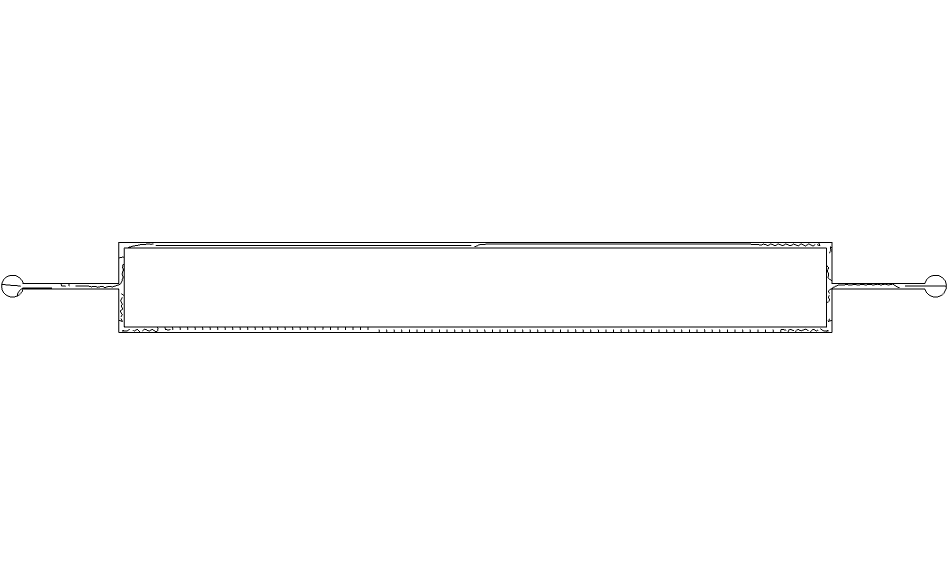
\includegraphics[width=\textwidth]{4.png}
\end{frame}
\begin{frame}{Results}{Electric potential}
    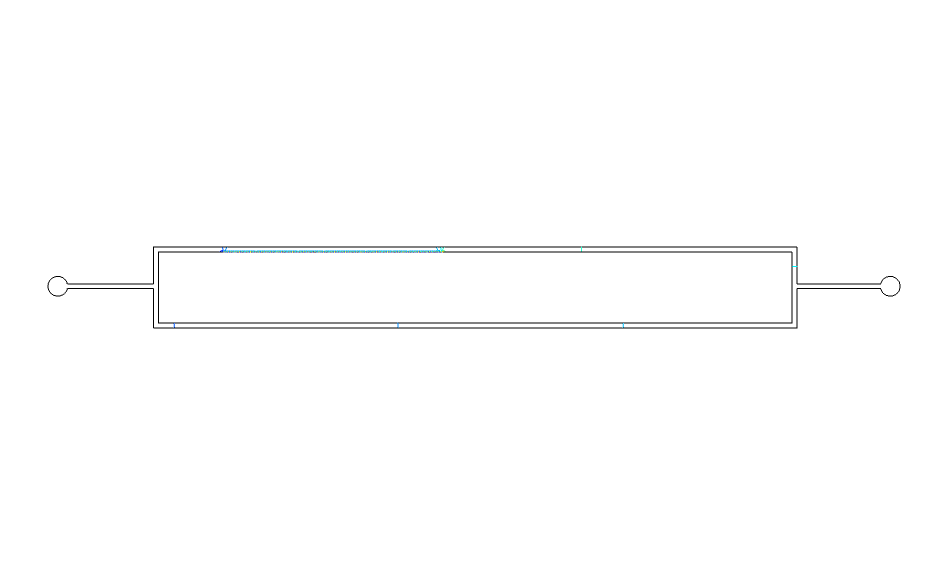
\includegraphics[width=\textwidth]{5.png}
\end{frame}
\begin{frame}{Results}{Electric potential}
    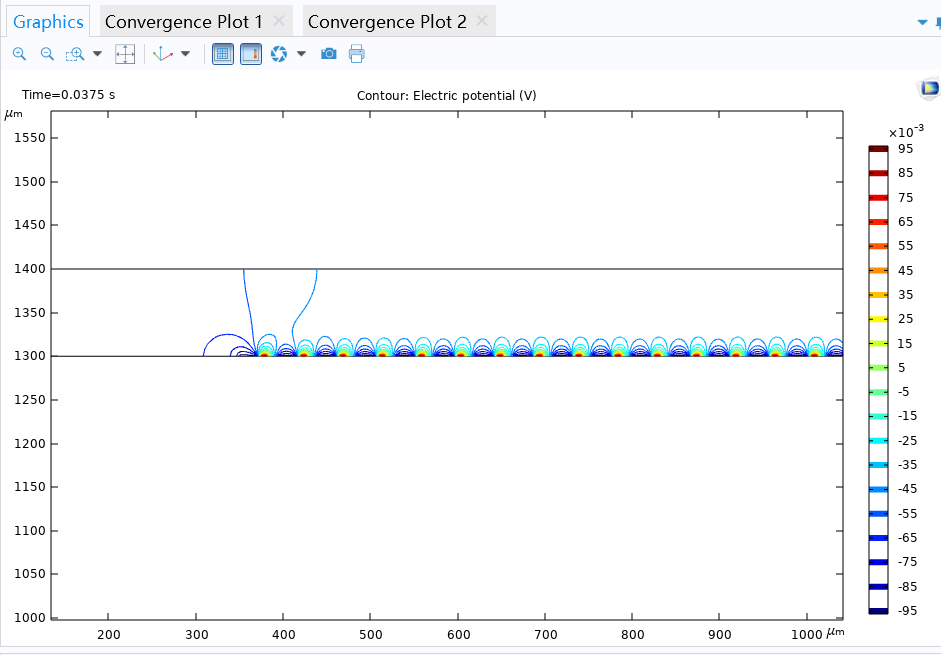
\includegraphics[width=\textwidth]{6.png}
\end{frame}
\section{Physical Model}
\begin{frame}{Physical Model}{Reference}
    Reference:\\
    Pham, Pascale, et al. "Numerical simulation of the electrical double layer based on the poisson-boltzmann models for ac electroosmosis flows." Excerpt from the Proceedings of the COMSOL Users Conference 2007 Grenoble. 2007.\\
    "Double layer (surface science)." Wikipedia, The Free Encyclopedia. 16 February 2021, 14:33 UTC. Wikimedia Foundation, Inc. 16 Mar. 2021. <https://en.wikipedia.org/wiki/Double\_layer\_(surface\_science)>.\\
    "Stern layer." SEAS Soft Matter Wiki. 9 December 2011, 03:46 UTC. 16 Mar. 2021. <http://soft-matter.seas.harvard.edu/index.php/Stern\_layer>\\
    González, Antonio, et al. "Fluid flow induced by nonuniform ac electric fields in electrolytes on microelectrodes. II. A linear double-layer analysis." Physical review E 61.4 (2000): 4019.
\end{frame}
\begin{frame}{Physical Model}
    \begin{itemize}
        \item Helmholtz: Predicted a constant differential capacitance; does not consider important factors including diffusion/mixing of ions in solution.
        \item Gouy-Chapman: The theory for a flat surface and a symmetrical electrolyte is usually referred to as the Gouy-Chapman theory.
              \[\sigma^d=-\sqrt{8\varepsilon_0\varepsilon_mCRT}\sinh{\frac{F\Psi^d}{2RT}}\]
              where $\sigma^d$ is the electric charge in the diffuse layer and $\Psi^d$ is the Stern potential.\\
              The Gouy-Chapman model fails for highly charged DLs (electrical double layers).
        \item Stern: Combining the Helmholtz model, giving an internal Stern layer, while some form a Gouy-Chapman diffuse layer.\\
              Assumes all significant interactions in the diffuse layer are Coulombic, and assumes dielectric permittivity to be constant throughout the double layer and that fluid viscosity is constant plane.
    \end{itemize}
\end{frame}
\begin{frame}{Physical Model}
    \begin{columns}[onlytextwidth]
        \begin{column}{0.45\textwidth}
            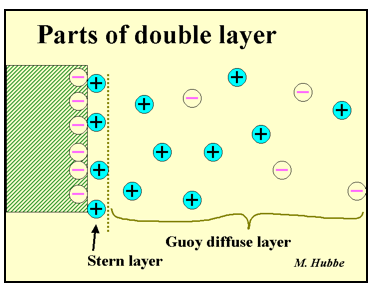
\includegraphics[width=\columnwidth]{7.png}
        \end{column}
        \begin{column}{0.45\textwidth}
            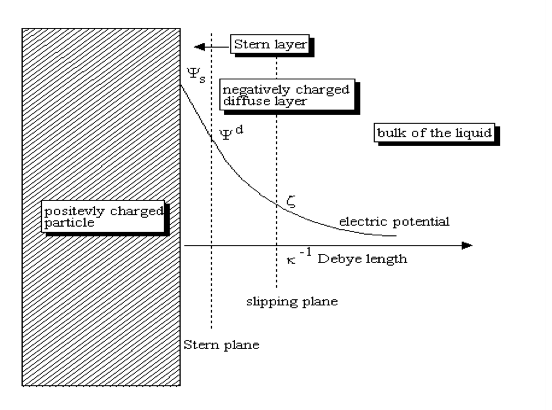
\includegraphics[width=\columnwidth]{8.png}
        \end{column}
    \end{columns}
    \begin{itemize}
        \item In the case when electric potential over DL is less than 25 mV, the so-called Debye-Huckel approximation holds.
              \[\Psi(r)=\Psi^d\frac{a}{r}\exp{(-\kappa(r-a))}\]
    \end{itemize}
\end{frame}
\begin{frame}{Physical Model}{COMSOL's approach}
    \begin{itemize}
        \item The Navier-Stokes equations for incompressible flow describe the flow in the channels:
              \[\rho\frac{\partial\bm{u}}{\partial t}-\nabla\cdot\eta\nabla\bm{u}+(\nabla\bm{u})^T+\rho\bm{u}\cdot\nabla\bm{u}+\nabla p=0\]
              \[\nabla\cdot\bm{u}=0\]
              Here $\eta$ denotes the dynamic viscosity (SI unit: kg/(m·s)), u is the velocity (SI unit: m/s), $\rho$ equals the fluid density (SI unit: kg/m3), and p refers to the pressure (SI unit: Pa).
        \item Total stress components normal to the boundary:
              \[\bm{n}\cdot[-p\bm{I}+\eta(\nabla\bm{u}+(\nabla\bm{u})^T)]=0\]
        \item Replace the thin electric double layer with the Helmholtz-Smoluchowski relation between the electroosmotic velocity and the tangential component of the applied electric field:
              \[\bm{u}=\frac{\varepsilon_w\zeta_0}{\eta}\nabla_TV\]
              $\varepsilon_w=\varepsilon_0\varepsilon_r$ denotes the fluid’s electric permittivity (F/m), $\zeta_0$ is the zeta potential at the channel wall (V). This equation applies only on the wall.
    \end{itemize}
\end{frame}
\begin{frame}{Physical Model}{COMSOL's approach}
    \begin{itemize}
        \item The balance equation for current density:
              \[\nabla\cdot(-\sigma\nabla V)=0\]
              where $\sigma$ denotes conductivity (S/m) and the expression within parentheses represents the current density (A/m$^2$).
        \item The normal component of the electric field is zero:
              \[-\sigma\nabla V\cdot\bm{n}=0\]
        \item (Not necessary) The convection-diffusion equation describes the concentration of the dissolved substances in the fluid:
              \[\frac{\partial c}{\partial t}+\nabla\cdot(-D\nabla c)=R-\bm{u}\cdot\nabla c\]
    \end{itemize}
\end{frame}
\begin{frame}
    \begin{center}
        Thanks!
    \end{center}
\end{frame}
\end{document}